% Chapter Template

\chapter{Conclusion} % Main chapter title

\label{Chapter7} % Change X to a consecutive number; for referencing this chapter elsewhere, use \ref{ChapterX}

\lhead{Chapter 7. \emph{Conclusions}} % Change X to a consecutive number; this is for the header on each page - perhaps a shortened title

%----------------------------------------------------------------------------------------
%	SECTION 1
%----------------------------------------------------------------------------------------

Low mass SUSY has been deeply constrained during run 1, however, the central motivation -- to stabilise the Higgs mass naturally -- remains. The LHC upgrade will provide significantly increased energies and luminosities. The effect this will have on SUSY production cross sections is shown in figure \ref{snow} \cite{ProjectedCx}. As can be seen the predicted probability for production of SUSY sparticles will be significantly increased. Any discovery of such events will rely on effective triggering. In chapter \ref{Chapter 6} studies into new algorithms for jets and pileup subtraction have been presented and shown to give significant advantages over the GCT. Further studies are required to optimise performance, however, these improvements should allow searches, such as $\alpha_T$, to maintain acceptance despite the increase in energy and luminosity. Cross triggers using quantities such as $\cancel{H_T}/{H_T}$ will be crucial in achieving this. If low mass SUSY is physical then the LHC upgrade and $\alpha_T$ will provide an excellent opportunity for discovery. 
\begin{figure}
\centering
    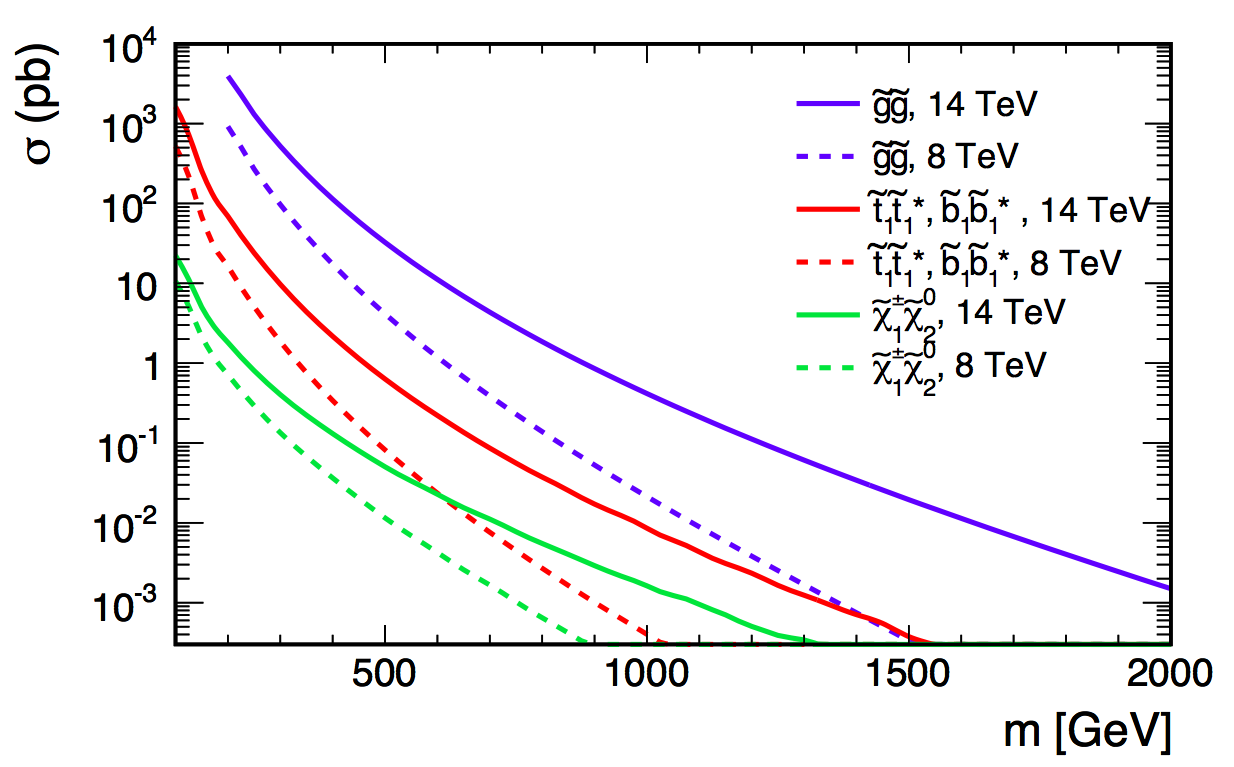
\includegraphics[width=0.7\textwidth]{Figures/snowmass.png}
  \caption{SUSY production cross sections at 14 TeV compared with 8TeV}
  \label{snow}
\end{figure}


